\documentclass[preprint,proceedings]{rmaa}


%%%
%%% Define any personal macros here
%%% 

% These are some I use in typesetting example code
\newcommand{\bs}{\textbackslash}
\newcommand{\CS}[1]{\texttt{\textbackslash #1}}
% roman subscripts in math
\newcommand{\Sub}[1]{_\mathrm{#1}}
% a command to specify possible linebreak points in an email address 
\newcommand{\D}{\discretionary{}{}{}}

%%%
%%% Article preamble commands (title, authors, abstract, etc.) 
%%% None of these produce any output themselves, they just set things 
%%% up for \maketitle
%%%

% This is only used for making the header for the preprint version
\SetYear{2016}
\SetConfTitle{XV LARIM}

% Please use mixed case here, since this title gets propagated onto
% the web page, ADS entry, etc. 
  \title{Laniakea in a cosmological context}
  
  \author{S. D. Hernandez-Charpak\altaffilmark{1} and
    J. E. Forero-Romero\altaffilmark{1}}  

\altaffiltext{1}{Departamento de F\'isica, Universidad de los Andes,
    Cra 1 18A-10, Bloque Ip, Bogot\'{a}, Colombia.
    (sd.hernandez204\D{}@uniandes\D{}.edu.\D{}co).}



  % List of authors used to construct table of contents
  \listofauthors{S. D. Hernandez-Charpak \& J. E. Forero-Romero}
  % Each author in Surname, Initials format, used in generating Author
  % Index entries.
  \indexauthor{Hernandez-Charpak, S. D.}
  \indexauthor{Forero-Romero, J. E.}


% No \abstract or \resumen for poster papers

% Keywords must be from the standard list and in alphabetical order. 
\addkeyword{cosmology: theory}
\addkeyword{cosmology: large-scale structure of the universe}


%%%
%%% Beginning of document proper
%%%
\begin{document}
% Typeset article header
\maketitle 
%%%Resumen en Español%%%
\boldabstract{Laniakea, nuestro superc\'{u}mulo local,
  fue definido a partir de observaciones recientes flujos c\'{o}smicos.
En este trabajo presentamos un estudio sobre simulaciones de N-cuerpos
con el fin de establecer la significancia de Laniakea en un contexto
cosmol\'{o}gico.  
Encontramos que superc\'{u}mulos similares en tama\~{n}o y estructura
a Laniakea son poco comunes en un contexto cosmol\'{o}gico amplio.} 

%%%Abstract%%%

\boldabstract{Laniakea, our local supercluster, 
  was defined by recent observationa of the local cosmic flow.
  In this work we present a study on large cosmological N-body
  simulations aimed at establishing the significance of Laniakea in a
  cosmological context.
  We find that superclusters similar in size and structure to Laniakea are
  relatively uncommon on a broader cosmological context.}

Tully et al. (2014) defined our home supercluster, Laniakea, as a region
region where the peculiar velocity flows converge. Laniakea is found
to be contained in a 160 Mpc diameter sphere.

We use a method to find superclusters in dark matter N-body
simulations and test it in a simulation of boxsize 350 Mpc. 

We base our method on the analysis of the eigenvalues $\lambda_1$,
$\lambda_2$ and  $\lambda_3$ of the velocity shear tensor $\Sigma _{\alpha\beta} = -\frac{1}{2 H_0} \left( \frac{\partial v_{\alpha}}{\partial
  x_{\beta}} + \frac{\partial v_{\beta}}{\partial x_{\alpha}}
\right)$ (Hoffman et al. 2012).

From these eigenvalues we compute the fractional anisotropy
(FA):
\begin{equation}
  \label{eq:njump}
   FA = \frac{1}{\sqrt{3}} \sqrt{\frac{( \left( \lambda_1 - \lambda_3 \right)^2 +
   \left( \lambda_2 - \lambda_3 \right)^2 + \left( \lambda_1 - \lambda_2 \right)^2 
   )}{\lambda^{2}_1 + \lambda^{2}_2 + \lambda^{2}_3}},
\end{equation}
which tells us whether a local collapse/expansion is anisotropic (FA=1) or
isotropic (FA=0).

We find regions with a negative velocity divergence below a
certain threshold of fractional anisotropy.
Figure
\ref{fig:simple} shows the number of superclusters with a given volumne.
Different curves correspond to different parameters in our
supercluster finding method. The first result is that large volume
superclusters are robust to changes in the algorithm.
The main result is that Laniakea is atypically larger than the
superclusters in our simulation. 

\begin{figure}[!t]
  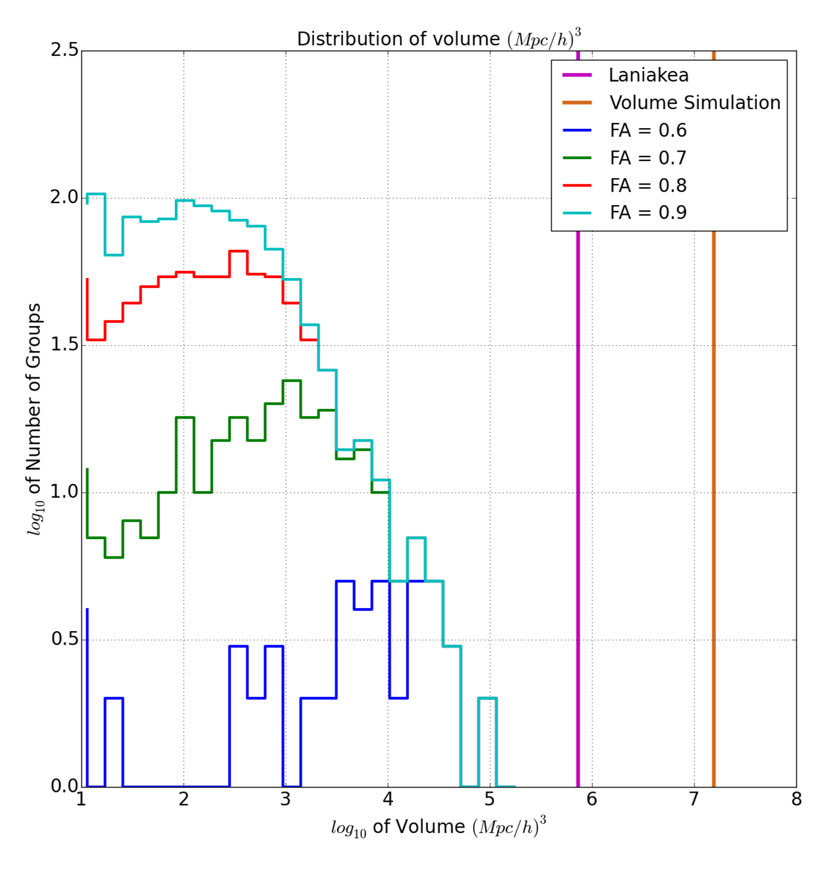
\includegraphics[width=\columnwidth]{SDHernandez_Final_Fig1}
  \caption{Abundances of superclusters with different volumes for
    different parameters in our algorithm.}
  \label{fig:simple}
\end{figure}


\begin{thebibliography}

\bibitem{1} R. Brent Tully, Hlne. Courtois, Yehuda Hoffman and Daniel Pomarde. 
{\em The Laniakea Supercluster of galaxies}, Nature, 513 (7516):71-73, September 2014 
 
\bibitem{2} Yehuda Hoffman, Ofer Metuki, Gustavo Yepes, Stefan Gottlöber, Jaime E. Forero-Romero, Noam I. Libeskind and Alexander Knebe. 
{\em A kinematic classification of the cosmic web}, Monthly Notices of the Royal Astronomical Society, 425: 2049–2057, August 2012

  
\end{thebibliography}

\end{document}
